\documentclass[a4paper]{article}

\usepackage[english]{babel}
\usepackage[utf8]{inputenc}
\usepackage{amsmath}
\usepackage{graphicx}
\usepackage{caption}
%\usepackage{subcaption}
%\usepackage{float}
\usepackage{natbib}
\usepackage{floatrow}
\usepackage[label font=bf,labelformat=simple]{subfig}
\floatsetup[figure]{style=plain,subcapbesideposition=top}
\usepackage[margin=1.25in]{geometry}
\captionsetup{labelfont=bf}
\usepackage{multirow}
\usepackage[table,xcdraw]{xcolor}



\title{Dysregulation of DNA Methylation in Human Intestinal Epithelial Organoids with Increasing Passage}

\author{Rachel Edgar}

\date{\today}

\begin{document}
\maketitle

\newpage


%\begin{table}[]
%\begin{tabular}{lllllllllll|l}
%\hline
%\rowcolor[HTML]{EFEFEF} 
%\cellcolor[HTML]{EFEFEF}                                     & \multicolumn{10}{l}{\cellcolor[HTML]{EFEFEF}\textbf{Passage}}                                                                       & \cellcolor[HTML]{EFEFEF}                                 \\
%\rowcolor[HTML]{EFEFEF} 
%\multirow{-2}{*}{\cellcolor[HTML]{EFEFEF}\textbf{Diagnosis}} & \textbf{1} & \textbf{2}  & \textbf{3} & \textbf{4} & \textbf{6} & \textbf{7} & \textbf{8} & \textbf{11} & \textbf{14} & \textbf{16} & \multirow{-2}{*}{\cellcolor[HTML]{EFEFEF}\textbf{Total}} \\ \hline
%\cellcolor[HTML]{EFEFEF}\textbf{Control}                     & 5          & 27          & 8          & 5          & 5          & 5          & 1          & 0           & 0           & 0           & \textbf{56}                                              \\
%\cellcolor[HTML]{EFEFEF}\textbf{Other GI}                    & 2          & 1           & 0          & 1          & 0          & 0          & 0          & 0           & 0           & 0           & \textbf{4}                                               \\
%\cellcolor[HTML]{EFEFEF}\textbf{IBD}                          & 0          & 7           & 1          & 1          & 0          & 2          & 2          & 2           & 4           & 1           & \textbf{20}                                              \\
%\cellcolor[HTML]{EFEFEF}\textbf{Total}                       & \textbf{7} & \textbf{35} & \textbf{9} & \textbf{7} & \textbf{5} & \textbf{7} & \textbf{3} & \textbf{2}  & \textbf{4}  & \textbf{1}  & \textbf{80}                                              \\ \hline
%\end{tabular}
%\end{table}
%


\begin{figure}
\begin{flushleft}
\sidesubfloat[]{\label{main:A}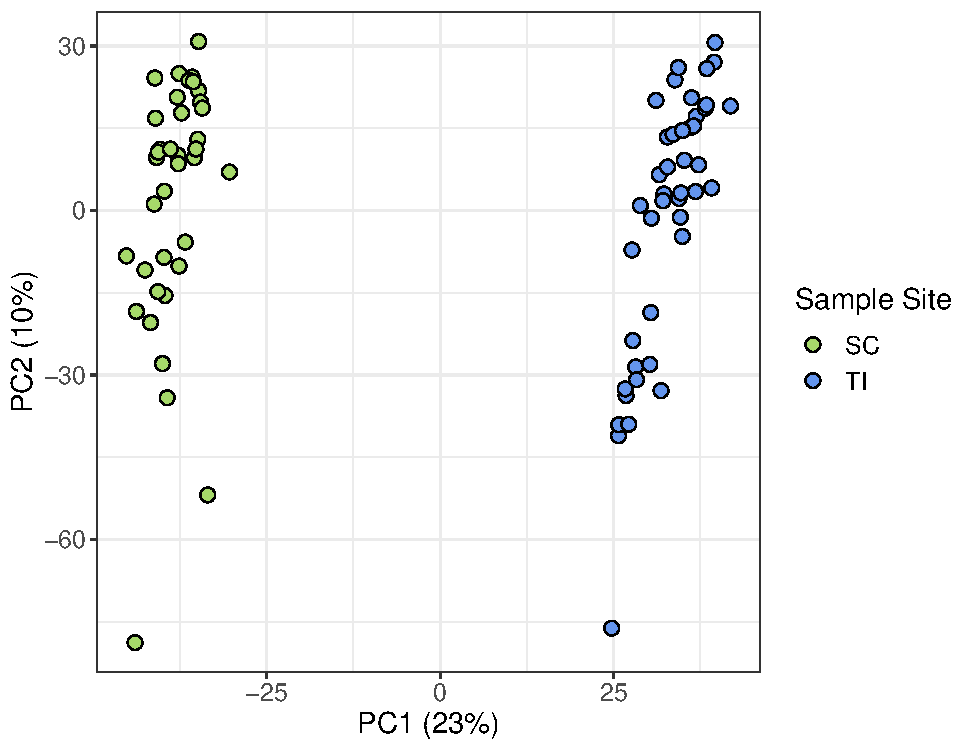
\includegraphics[width=0.71\textwidth]{../figs/PC1_PC2_organoid.pdf}}
\hfil
\sidesubfloat[]{\label{main:B}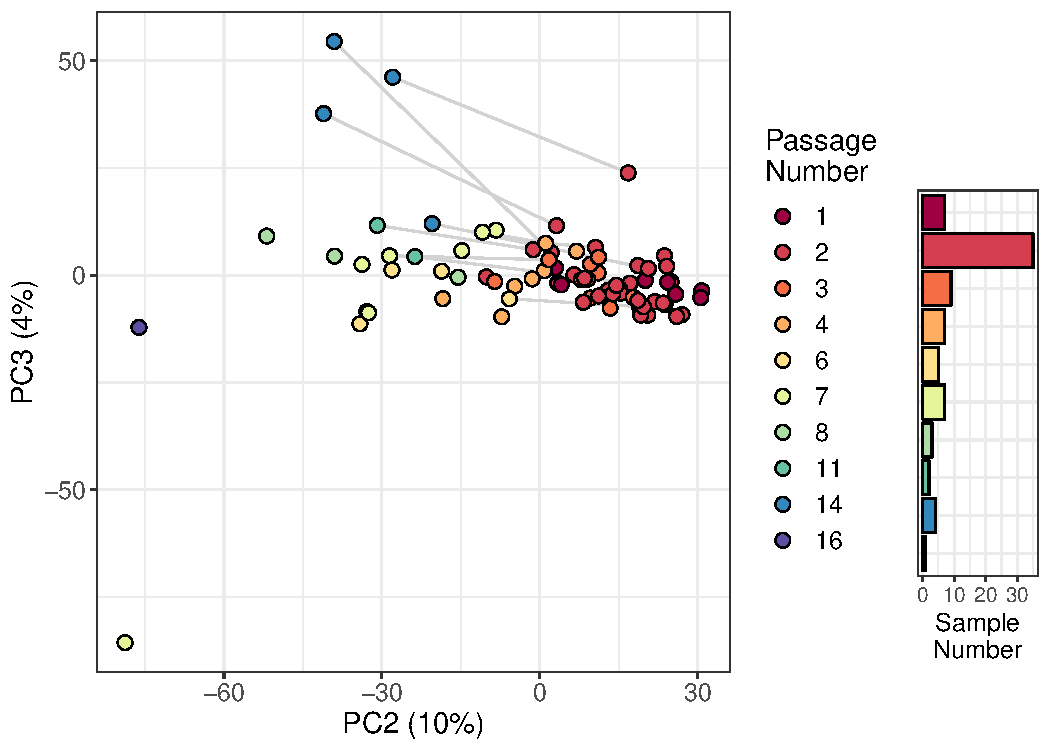
\includegraphics[width=0.80\textwidth]{../figs/PC2_PC3_organoid.pdf}}

\caption{\textbf{Sampling site of origin and organoid passage number are associated to the main components of DNAm variation.} (a) PC1 and PC2 are plotted for each sample. Samples are coloured by the sampling site of origin. (b) PC2 and PC3 are plotted for each sample. Samples are coloured by passage number. Lines connect samples derived from the same patient, but where organoids were cultured to a different number of passages. The histogram in the legend shows the distribution of passage numbers across the cohort.}
\label{fig:main}
\end{flushleft}
\end{figure}






%
\begin{figure}
\begin{flushleft}

\begin{minipage}{.45\linewidth}
\sidesubfloat[]{\label{main:a}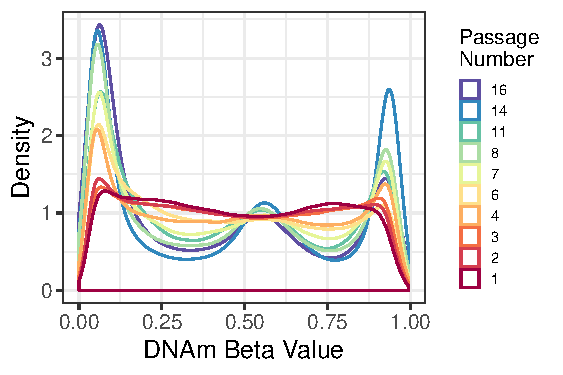
\includegraphics[width=1\textwidth]{../figs/Passage_variable_CpGs.pdf}}
\end{minipage}%
\hspace{5mm}
\begin{minipage}{.45\linewidth}
\centering
\sidesubfloat[]{\label{main:c}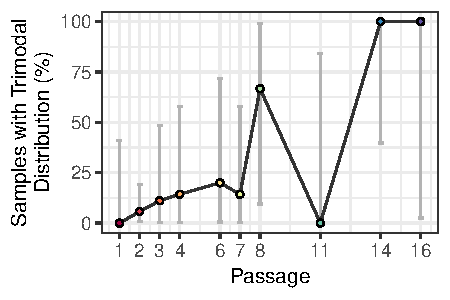
\includegraphics[width=1\textwidth]{../figs/Mixture_model_ratio_threshold_maximize.pdf}}
\end{minipage}\par\bigskip
\centering
\sidesubfloat[]{\label{main:b}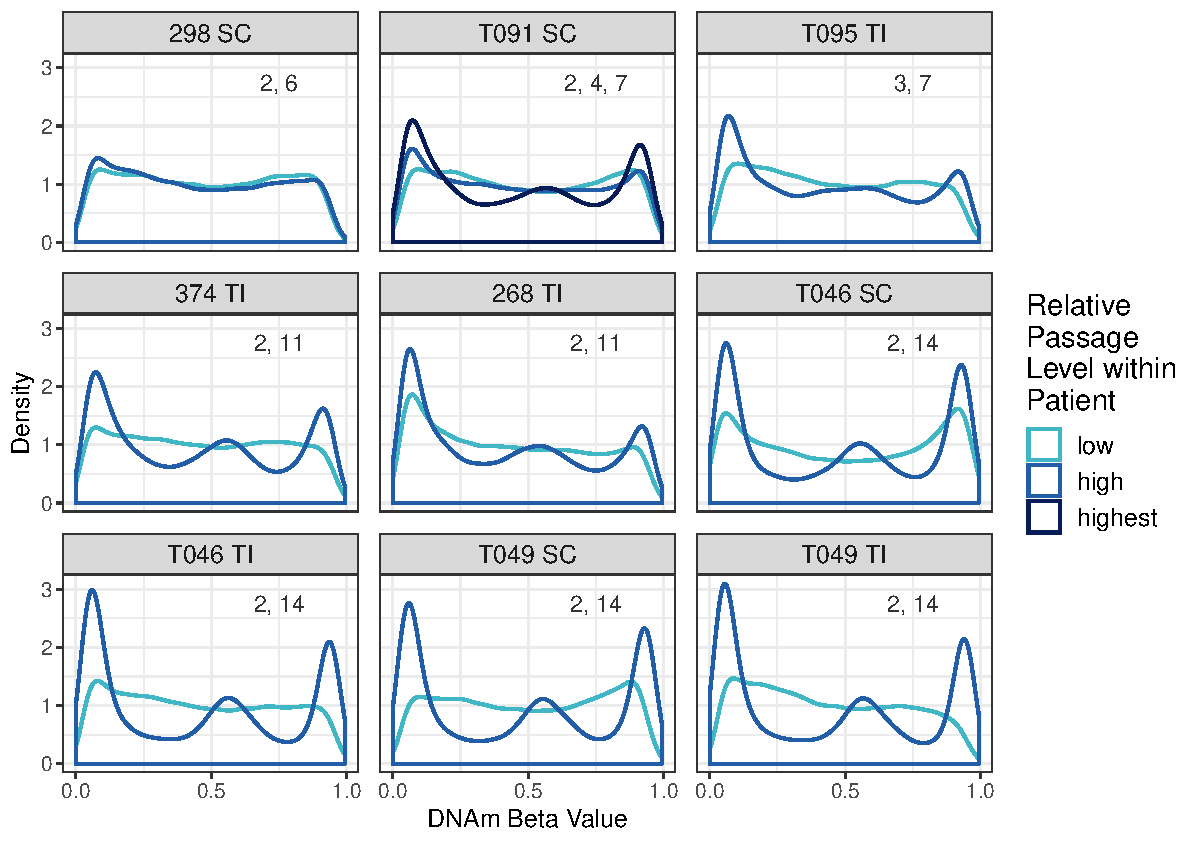
\includegraphics[width=1\textwidth]{../figs/Passage_paried_beta.pdf}}

\caption{\textbf{DNAm beta value distributions are trimodal for high passage samples but bimodal for low passage samples.} All beta distributions displayed are for the 51,545 most variable CpGs. (a) Beta value distributions for all samples at a given passage number. Curves are coloured by the passage number. (b) The percent of samples considered trimodal. Points are coloured by passage and the bars around each point represent the confidence interval for that percent. (c) Beta value distributions for samples derived from the same patient but cultured to a different number of passages. Plots are labelled with the patient ID number, sampling site of origin and the passage number of each sample derived from that patient and sampling site. Curves are coloured by high or low passage relative to the other sample(s).}
\label{fig:main}
\end{flushleft}
\end{figure}





\begin{figure}
\begin{centering}
\sidesubfloat[]{\label{main:A}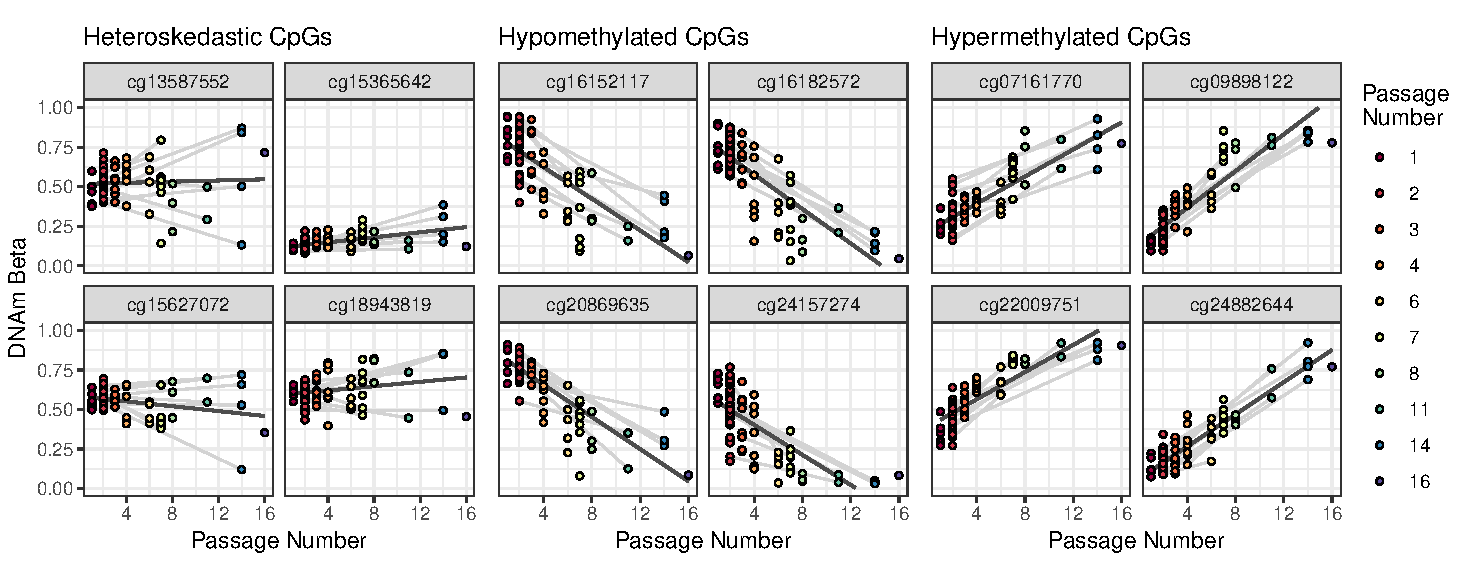
\includegraphics[width=1\textwidth]{../figs/Passage_representative_CpGs_FDR.pdf}}
\hfil
\sidesubfloat[]{\label{main:B}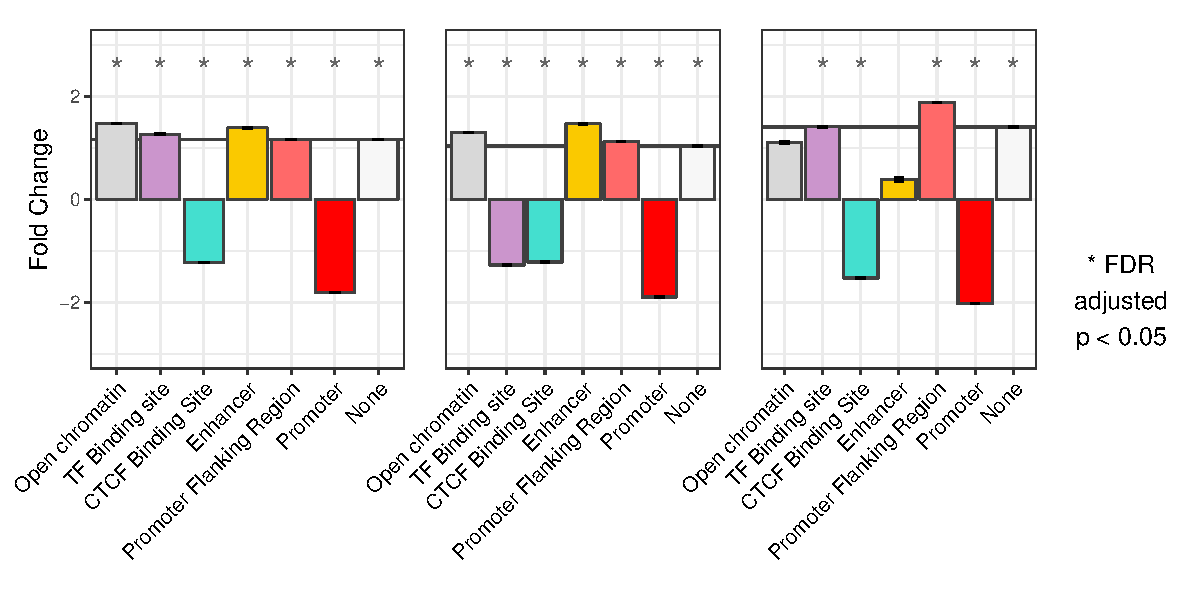
\includegraphics[width=1\textwidth]{../figs/Passage_hetero_hypo_hyper_reg_CpGs_FDR_background015.pdf}}
\hfil
\sidesubfloat[]{\label{main:B}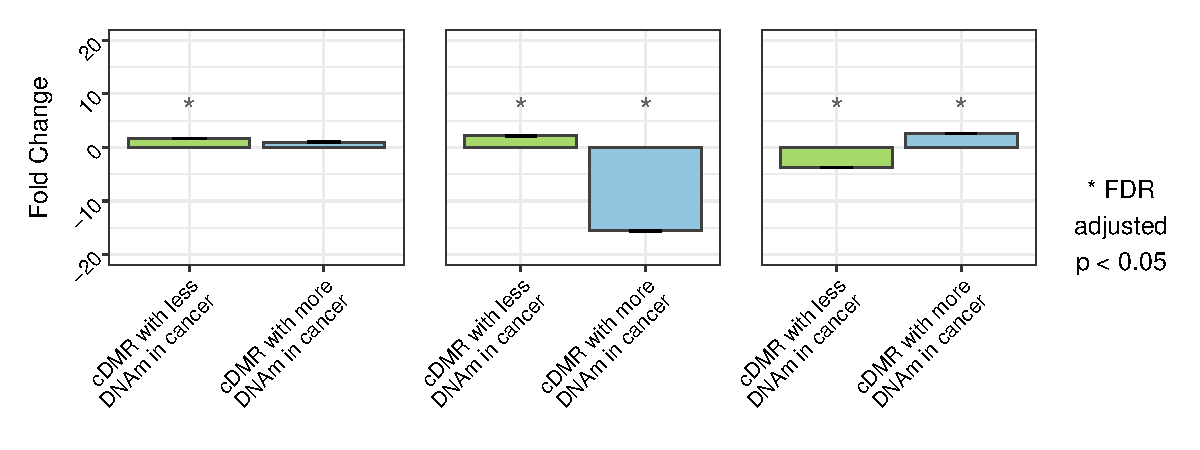
\includegraphics[width=1\textwidth]{../figs/Passage_hetero_hypo_hyper_DMR_CpGs_FDR_background015.pdf}}

\caption{\textbf{Passage affects DNAm in specific regions of the genome.} (a) Representative CpGs with DNAm significantly associated to passage. CpGs were selected that are either significantly heteroskedastic with passage or are differentially DNA methylated and either lose (hypomethylated) or gain (hypermethylated) DNAm with increasing passage. Samples are coloured by passage number and grey lines connect samples derived from the same patient. Regression lines between passage and DNAm are in black. (b) Fold change between the number of passage associated CpGs in regulatory genomic features and expected number based on the EPIC array background. Standard error bars around the mean fold change are for the error across 1,000 random samplings.(c) Fold change between the number of passage associated CpGs in cDMRs and expected number based on the EPIC array background. Standard error bars around the mean fold change are for the error between 1,000 random samplings.}

\label{fig:main}
\end{centering}
\end{figure}


\end{document}